\documentclass{article}
\usepackage{fullpage}
\usepackage{graphics}

\parskip 0.2cm
\parindent 0cm

\newcommand{\fname}[1]{{\tt #1}}
\newcommand{\code}[1]{{\tt #1}}

\title{Architecture for High-Frequency Sampling}
\author{The TASK team}

\begin{document}

\maketitle

\section{Introduction}

This document presents the architecture for high-frequency sample
collection in TinyOS and TASK. We define a \emph{sample} as $n$
measurements obtained from one or more sensors at some frequency $f$. These
samples will be processed locally and/or sent over the radio to other motes
or a base station. We are targeting applications where the frequency $f$ is
too high for real-time processing of the measurement. Therefore we assume
that there is significant time between the collection of each sample, and
that the latency in processing or sending a sample is not a significant
issue.

\section{Overall Architecture}

\begin{figure}[t]
  \resizebox{3in}{3in}{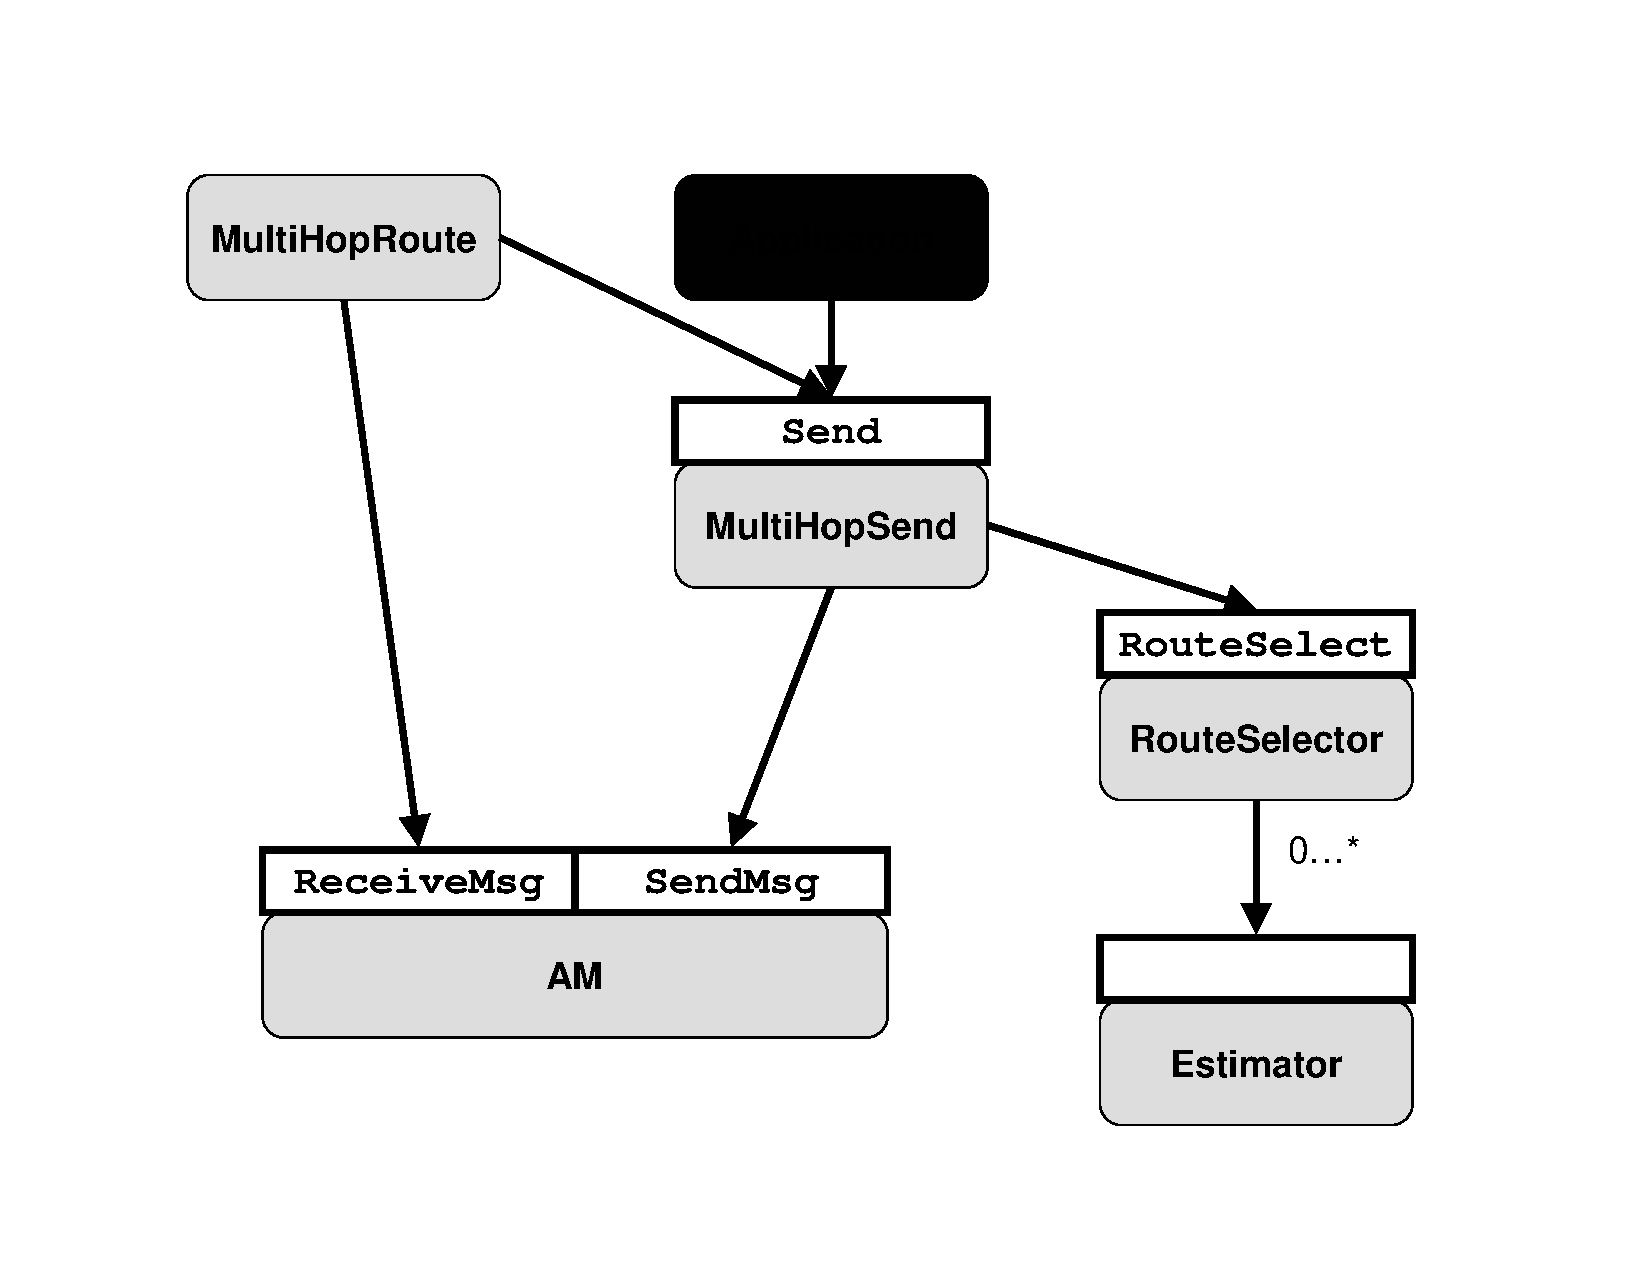
\includegraphics{arch.png}}
  \caption{Architecture for sample collection and processing}
  \label{fig:arch}
\end{figure}

The sampling architecture we propose is passive: its behaviour is driven by
external requests to collect, send or receive a sample. The overall
architecture is shown in Figure~\ref{fig:arch}. We start with a brief
overview of each component.

\paragraph{Sampler} The sampler collects a sample and places it in an
identifiable part of the storage. Depending on hardware support and
sampling frequency, the sampler may need to ``take over'' the mote
while sampling.

\paragraph{Storage} The storage is used to store samples collected by
the sampler and received from other motes. Each item in storage is composed
of some metadata and the uninterpreted sample data.

\paragraph{Send, Receive}: These components can send and receive storage
items when requested.

Not all components will be present in all applications: for instance, if
there is no multihop sample transmission, then there will be no Receive,
and the storage (probably) only needs to store a single sample. The
implementation of this architecture must be flexible, allowing use of 
different samplers, storage components, send and receive protocols, etc.

\section{Sampling}

Sampling may be performed on the mote, or on an external board (e.g.,
Crossbow's MDA400). In either case, it is controlled using the
\code{Sampling} interface shown in Appendix~\ref{intf:sampling}. If
the sampling is performed on the mote, it will output its data using
the \code{LogData} interface shown in Appendix~\ref{intf:logdata}.
Integrated sampling/storage solutions like the MDA400 do not
expose a specific storage interface. [[Open issue: how does the MDA400
storage fit in to the storage model below?]]

\subsection{On-mote Sampling}

The architecture for on-mote sampling is shown in
Figure~\ref{fig:sampling}, it includes the following components:

\begin{itemize}
  
\item Sample: main sampling component: collects and logs n samples at a 
specified interval, to storage. Sample provides the Sampling interface
described in the attached Sampling.nc file, collects samples via an
ADC interface and logs data via the LogData interface and a special-purpose
fastAppend command.

\item MicroTimer: high-precision timer (support intervals $<1$ms)

\item ByteEEPROM: shared access to the flash via AllocationReq, WriteData,
ReadData and LogData interfaces. The flash is divided into fixed-size
chunks, allocated at boot time via the AllocationReq interface. Each chunk
is identified by an id which is used to parameterise ByteEEPROM's
interfaces. The LogData interface  (see the attached LogData.nc file)
is designed for maximum write performance.

\item BufferedLog: ByteEEPROM's LogData interface is not optimised for
small writes. BufferedLog remedies this problem by providing a LogData
interface, along with a fastAppend command optimised for small writes.

\end{itemize}

Sample's flow is as follows:
\begin{enumerate}
\item when a prepare command is received, it erases the storage via the 
LogData interface.
\item when start is called, it first calls ExternalShutdown.stop to stop any
services that should not run during sampling, then starts sampling.
\item when sampling is complete, it calls LogData.sync to ensure all data
is in the flash, and ExternalShutdown.start to restart the stopped services
\end{enumerate}

The core of the sampling process is essentially the Sample, MicroTimer
and BufferedLog components. These provide a Sampling interface, and
depend on the following:
\begin{itemize}
\item an ADC interface to get samples
\item a LogData interface to store sampled data
\item an ExternalShutdown (StdControl) interface to start/stop other services
during sampling
\end{itemize}

The user of this sampling core is responsible for:
\begin{itemize}
\item connecting the ADC interface to the appropriate sensor
\item allocating a correctly-sized area of storage, and connecting the LogData
interface to that storage
\item connecting ExternalShutdown to appropriate services (most obviuously
the radio and Timer)
\end{itemize}

Error checking (for storage overflow, inappropriate sampling rates, 
incorrect interface usage, etc) is currently either absent or performed
at runtime. This will not change.

The \code{ADC} interface will be replaced by a more general \code{Sensing}
interface to support samples where each measurement gets data from several
sensors.

The \code{BufferedLog}, \code{ByteEEPROM} combination can be replaced by
another storage component.

\section{Storage}

The storage components should support the same interfaces as
\code{ByteEEPROM}. This choice means that the number and size of storage
blocks is fixed at boot time. [[Open Issue: is this acceptable?]]

\section{Sample Transmission}

The underlying model for sample transmission is a custody transfer. Once a
mote has reliably sent a sample to the next stage in the network it can
forget about it and reuse any associated storage space. There are thus two
parts to sample transmission. First, the design and implementation of a
reliable single-sample, single-hop transmission protocol (this is
essentially a ``large object'' transmission protocol, and should be shared
with other system components that also need it).  Second is the design of
the network infrastructure and the scheduling of sample transmission. There
are several obvious choices:
\begin{itemize}
\item A single-hop network. Each mote sends its samples to heavier-duty
(e.g., PCs with Ethernet) nodes which are then responsible for them. The
network must still schedule communication from each mote to allow all
samples to be extracted.

\item A multi-hop network. Motes send their samples either to heavier-duty
nodes (at the ``edge'' of the network), or to other motes. The scheduling
problem is harder, as it places more demands on bandwidth in the mote network,
and it must avoid overloading (both in bandwidth and storage) the intermediate
motes in the multi-hop network.
\end{itemize}

We expect the most interesting research issues to arise in this area\ldots

\section{Other Issues}

\paragraph{Power}
Power management is obviously of major importance. Each component should
therefore support the \code{StdControl} interface so that it can be
switched to a low-power mode. Beyond this basic level, power usage will be
mainly determined by the sample (size, frequency, interval between samples)
and network (protocol, size and organisation, etc) characteristics which
are beyond the scope of this document.

\appendix
\small

\section{Sampling interface}
\label{intf:sampling}

\begin{verbatim}
// $Id: arch.tex,v 1.1 2004/02/18 22:17:54 idgay Exp $
/*                                                                      tab:4
 * "Copyright (c) 2000-2003 The Regents of the University  of California.  
 * All rights reserved.
 *
 * Permission to use, copy, modify, and distribute this software and its
 * documentation for any purpose, without fee, and without written agreement is
 * hereby granted, provided that the above copyright notice, the following
 * two paragraphs and the author appear in all copies of this software.
 * 
 * IN NO EVENT SHALL THE UNIVERSITY OF CALIFORNIA BE LIABLE TO ANY PARTY FOR
 * DIRECT, INDIRECT, SPECIAL, INCIDENTAL, OR CONSEQUENTIAL DAMAGES ARISING OUT
 * OF THE USE OF THIS SOFTWARE AND ITS DOCUMENTATION, EVEN IF THE UNIVERSITY OF
 * CALIFORNIA HAS BEEN ADVISED OF THE POSSIBILITY OF SUCH DAMAGE.
 * 
 * THE UNIVERSITY OF CALIFORNIA SPECIFICALLY DISCLAIMS ANY WARRANTIES,
 * INCLUDING, BUT NOT LIMITED TO, THE IMPLIED WARRANTIES OF MERCHANTABILITY
 * AND FITNESS FOR A PARTICULAR PURPOSE.  THE SOFTWARE PROVIDED HEREUNDER IS
 * ON AN "AS IS" BASIS, AND THE UNIVERSITY OF CALIFORNIA HAS NO OBLIGATION TO
 * PROVIDE MAINTENANCE, SUPPORT, UPDATES, ENHANCEMENTS, OR MODIFICATIONS."
 *
 * Copyright (c) 2002-2003 Intel Corporation
 * All rights reserved.
 *
 * This file is distributed under the terms in the attached INTEL-LICENSE     
 * file. If you do not find these files, copies can be found by writing to
 * Intel Research Berkeley, 2150 Shattuck Avenue, Suite 1300, Berkeley, CA, 
 * 94704.  Attention:  Intel License Inquiry.
 */
/** 
 * A sampling interface. Note that where sampling data is collected and
 * how that data is recovered is up to each sampling component
 */
interface Sampling {
  /**
   * Prepare to peform sampling. 
   * @param interval The interval in microseconds between samples
   * @param count The number of samples to collect
   * @param circular TRUE for circular sampling (sampling will only
   *   end when stop is called.
   * @return If the result is SUCCESS, <code>ready</code> will be signaled
   *   If the result is FAIL, no sampling will happen.
   */
  command result_t prepare(uint32_t interval, uint32_t count, bool circular);

  /**
   * Report if sampling can be started
   * @param ok SUCCESS if sampling can be started by calling 
   *   <code>start</code>, FAIL otherwise
   * @return Ignored
   */
  event result_t ready(result_t ok);

  /** 
   * Start sampling requested by previous <code>prepare</code>
   * @return SUCCESS if sampling started (<code>done</code> will be signaled
   *   when it complates), FAIL if it didn't.
   */
  command result_t start();

  /** 
   * Stop sampling started by earlier <code>start</code>
   * @return SUCCESS if sampling can be stopped (<code>done</code> will 
   *   be signaled shortly), FAIL if it can't.
   */
  command result_t stop();

  /**
   * Report sampling completion
   * @param ok SUCCESS if sampling was succesful, FAIL if it failed. Failure
   *   may be due to the sampling interval being too short or to a data
   *   logging problem.
   * @param sampledBytes Number of bytes of sampling data collected
   * @return Ignored
   */
  event result_t done(result_t ok, uint32_t sampledBytes);
}
\end{verbatim}

\section{LogData interface}
\begin{verbatim}
// $Id: arch.tex,v 1.1 2004/02/18 22:17:54 idgay Exp $
/*                                                                      tab:4
 * "Copyright (c) 2000-2003 The Regents of the University  of California.  
 * All rights reserved.
 *
 * Permission to use, copy, modify, and distribute this software and its
 * documentation for any purpose, without fee, and without written agreement is
 * hereby granted, provided that the above copyright notice, the following
 * two paragraphs and the author appear in all copies of this software.
 * 
 * IN NO EVENT SHALL THE UNIVERSITY OF CALIFORNIA BE LIABLE TO ANY PARTY FOR
 * DIRECT, INDIRECT, SPECIAL, INCIDENTAL, OR CONSEQUENTIAL DAMAGES ARISING OUT
 * OF THE USE OF THIS SOFTWARE AND ITS DOCUMENTATION, EVEN IF THE UNIVERSITY OF
 * CALIFORNIA HAS BEEN ADVISED OF THE POSSIBILITY OF SUCH DAMAGE.
 * 
 * THE UNIVERSITY OF CALIFORNIA SPECIFICALLY DISCLAIMS ANY WARRANTIES,
 * INCLUDING, BUT NOT LIMITED TO, THE IMPLIED WARRANTIES OF MERCHANTABILITY
 * AND FITNESS FOR A PARTICULAR PURPOSE.  THE SOFTWARE PROVIDED HEREUNDER IS
 * ON AN "AS IS" BASIS, AND THE UNIVERSITY OF CALIFORNIA HAS NO OBLIGATION TO
 * PROVIDE MAINTENANCE, SUPPORT, UPDATES, ENHANCEMENTS, OR MODIFICATIONS."
 *
 * Copyright (c) 2002-2003 Intel Corporation
 * All rights reserved.
 *
 * This file is distributed under the terms in the attached INTEL-LICENSE     
 * file. If you do not find these files, copies can be found by writing to
 * Intel Research Berkeley, 2150 Shattuck Avenue, Suite 1300, Berkeley, CA, 
 * 94704.  Attention:  Intel License Inquiry.
 */
/*
 * Authors:             David Gay
 * Date last modified:  7/15/03
 *
 */

/** 
 * This interface is used to provide efficient, byte level logging to
 * a region of memory/flash/etc (the actual region is specified through
 * some other mechanism, e.g., in ByteEEPROM by providing a parameterised
 * LogData interface). Unlike the WriteData interface, the data written
 * via append is only guaranteed to be present in the region once sync
 * has completed.
 *
 * Note: this interface is purposefully restrictive to allow logging to
 * be as fast as possible. Calls to LogData must not be interspersed
 * with calls to WriteData on the same area of memory/flash/etc
 * (ReadData is fine). WriteData can be called after syncDone returns.
 * This interface is currently used by ByteEEPROM
 * @author David Gay
 */

interface LogData
{
  /** Erase region, reset append pointer to beginning of region
   * @return FAIL if erase request was refused. Otherwise SUCCESS
   *   is returned and <code>eraseDone</code> will be signaled.
   */
  command result_t erase();

  /**
   * Report erase completion.
   * @param success FAIL if erase failed, in which case appends are not allowed.
   * @return Ignored.
   */
  event result_t eraseDone(result_t success);

  /** Append bytes to region (erase must be called first)

   * @return FAIL if appends are not allowed (erase failed or sync has been
   * called). If the result is SUCCESS, <code>appendDone</code> will be signaled.
   */
  command result_t append(uint8_t* data, uint32_t numBytes);

  /**
   * Report append completion.
   * @param data Address of data written
   * @param numBytesWrite Number of bytes written
   * @param success SUCCESS if write was successful, FAIL otherwise
   * @return Ignored.
   */
  event result_t appendDone(uint8_t* data, uint32_t numBytes, result_t success);

  /**
   * Report current append offset.
   * @return the current append offset, or (uint32_t)-1
      if appends are not allowed (after sync or before erase)
   */
  command uint32_t currentOffset();

  /** 
   * Ensure all data written by append is committed to flash.
   * Once sync is called, no more appends are allowed.
   * @return FAIL if sync request is refused. If the result is SUCCESS
   * the <code>syncDone</code> event will be signaled.
   */
  command result_t sync();

  /**
   * Report sync completion.
   * @param success FAIL if sync failed, SUCCESS otherwise.
   * @return Ignored.
   */
  event result_t syncDone(result_t success);
}

\end{verbatim}

\end{document}
